\chapter*{Ausarbeitung}

\section*{Aufgabe 1 Somigliana-Pizzetti-Normalpotential}

In der ersten Aufgabe dieser Übung soll aus der geozentrischen Gravitationskonstante $GM$, den Halbachsen $a$, $b$ des Referenzellipsoides und aus der Rotationsgeschwindigkeit der Erde $\omega$ der konstante Potentialwert $U_0$ des Somigliana-Pizzetti-Referenzpotentials auf dem Referenzellipsoid bestimmt werden. \\

Die exakte Darstellung des Normalpotentials in ellipsoidischen Koordinaten sieht wie folgt aus:

\begin{align}
U^{Ell}(\lambda,\beta,u) = \left(U_0 - \dfrac{\omega^2 a^2}{3}\right) \dfrac{Q_{0,0}^{*}\left(\dfrac{u}{E}\right)}{{Q_{0,0}^{*}\left(\dfrac{b}{E}\right)}} + \dfrac{\omega^2 a^2 Q_{2,0}^{*}\left(\dfrac{u}{E}\right)}{3 Q_{2,0}^{*}\left(\dfrac{b}{E}\right)} P_{2,0}(\sin \beta)
\end{align}

mit $E = \sqrt{a^2 - b^2}$, und 

\begin{align}
Q_{0,0}^{*}\left(\dfrac{u}{E}\right) &= \arctan \left(\dfrac{E}{u}\right) \\
Q_{2,0}^{*}\left(\dfrac{b}{E}\right) &= \dfrac{1}{2} \left[\left(3 \left(\dfrac{b}{E}\right)^2+1\right) \text{arccot} \left(\dfrac{b}{E}\right)-3 \left(\dfrac{b}{E}\right)\right]
\end{align}

Die Darstellung des Normalpotentials in sphärischen Koordinaten lautet: 

\begin{align}
U^{Sph}(\lambda,\varphi,r)= \dfrac{GM}{r} \left[1-\sum_{n=1}^{L} \left(\dfrac{a}{r}\right)^{2n} J_{2n} P_{2n} (\sin \varphi)\right] + \dfrac{\omega^2}{2} r^2 \cos^2 \varphi
\end{align}

mit 

\begin{align*}
J_2 &= \dfrac{e^2}{3} \left(1-\dfrac{2}{15} \dfrac{e'\hat{m}}{q_0}\right) \\
J_{2n} &= (-1)^{n+1} \dfrac{3e^{2n}}{(2n+1)(2n+3)} \left(1-n+5n \dfrac{J_2}{e^2}\right) ~~~~~ n > 1 
\end{align*}

Des Weiteren gilt:

\begin{gather*}
e = \dfrac{E}{a}, ~~~~~ e'= \dfrac{E}{b} \\
\hat{m} = \dfrac{\omega^2 a^2 b }{GM}, ~~~~~ q_0 = Q_{2,0}^{*} \left(\dfrac{b}{E}\right)
\end{gather*}

Im ersten Schritt gilt es beide Darstellungen des Potentials mit dem Radius $r$ zu multiplizieren und folglich die Grenzwerte 	\dq im Unendlichen\dq zu betrachten. Aus der Grenzwertbetrachtung $\lim_{r \rightarrow \infty}$ der sphärischen Koordinaten kann folgendes festgestellt werden:

\begin{align*}
\lim_{r \rightarrow \infty} r \cdot U^{Sph}(\lambda,\varphi,r) = \lim_{r \rightarrow \infty} r \cdot \left(\dfrac{GM}{r} \left[1-\sum_{n=1}^{L} \left(\dfrac{a}{r}\right)^{2n} J_{2n} P_{2n} (\sin \varphi)\right] + \dfrac{\omega^2}{2} r^2 \cos^2 \varphi\right) = GM
\end{align*}

Der Grenzwert liegt bei $GM$. Dementsprechend kann davon ausgegangen werden, dass für die Grenzwertbetrachtung bei ellipsoidischen Koordinaten das gleiche gilt:

\begin{align*}
\lim_{r \rightarrow \infty} r \cdot U^{Ell}(\lambda,\beta,u) = \lim_{r \rightarrow \infty} r \cdot \left(\left(U_0 - \dfrac{\omega^2 a^2}{3}\right) \dfrac{Q_{0,0}^{*}\left(\dfrac{u}{E}\right)}{{Q_{0,0}^{*}\left(\dfrac{b}{E}\right)}} + \dfrac{\omega^2 a^2 Q_{2,0}^{*}\left(\dfrac{u}{E}\right)}{3 Q_{2,0}^{*}\left(\dfrac{b}{E}\right)} P_{2,0}(\sin \beta)\right) = GM
\end{align*}

Im Anschluss geht es darum einen Zusammenhang zwischen den fünf definierenden Größen ($a,b,\omega,GM,U_0$) zu erreichen, indem kleine Größen vernachlässigt werden. Anmerkung: $u$ verhält sich genauso wie $r$. Zunächst müssen allerdings die Funktionen $Q_{0,0}^{*}$ und $Q_{2,0}^{*}$ durch die ersten Terme ihrer Taylorreihen approximiert werden. Wie oben beschrieben gilt: 

\begin{align*}
Q_{0,0}^{*} = \arctan \left(\dfrac{E}{u}\right)
\end{align*}

Die Reihenentwicklung des $\arctan$ lautet im Bereich $-1 < x < 1$:  

\begin{align*}
\arctan(x) = x- \dfrac{x^3}{3} + \dfrac{x^5}{5} + ...
\end{align*}

Durch einsetzen von $\dfrac{E}{u}$ in $\arctan(x)$ ergibt sich also: 

\begin{align*}
Q_{0,0}^{*} \left(\dfrac{u}{E}\right) = \left(\dfrac{E}{u}\right)- \dfrac{\left(\dfrac{E}{u}\right)^3}{3}+ \dfrac{\left(\dfrac{E}{u}\right)^5}{5} + ...
\end{align*}

\begin{align*}
\approx \left(\dfrac{E}{u}\right) - \dfrac{1}{3} \cdot \left(\dfrac{E}{u}\right)^3 + \dfrac{1}{5} \left(\dfrac{E}{u}\right)^5 
\end{align*}

Gleichermaßen wird $\dfrac{E}{b}$ eingesetzt:

\begin{align*}
Q_{0,0}^{*} \left(\dfrac{b}{E}\right) \approx \left(\dfrac{E}{b}\right) - \dfrac{1}{3} \cdot \left(\dfrac{E}{b}\right)^3 + \dfrac{1}{5} \left(\dfrac{E}{b}\right)^5
\end{align*}

Für $Q_{2,0}^{*}$ gilt: 

\begin{align*}
Q_{2,0}^{*}\left(\dfrac{b}{E}\right) = \dfrac{1}{2} \left[\left(3 \left(\dfrac{b}{E}\right)^2+1\right) \text{arccot} \left(\dfrac{b}{E}\right)-3 \left(\dfrac{b}{E}\right)\right]
\end{align*}

Daraus ergibt sich für die Approximation: 

\begin{align*}
Q_{2,0}^{*}\left(\dfrac{u}{E}\right) = \dfrac{1}{2} \left[\left(3 \left(\dfrac{u}{E}\right)^2+1\right) \cdot \left(\left(\dfrac{E}{u}\right)-\dfrac{\left(\dfrac{E}{u}\right)^3}{3}+\dfrac{\left(\dfrac{E}{u}\right)^5}{5}+...\right)-3 \left(\dfrac{u}{E}\right)\right]
\end{align*}

\begin{align*}
\approx \dfrac{2}{15} \left(\dfrac{E}{u}\right)^3 + \dfrac{1}{10} \left(\dfrac{E}{u}\right)^5
\end{align*}

Genauso wird berechnet: 

\begin{align*}
Q_{2,0}^{*}\left(\dfrac{b}{E}\right) = \dfrac{1}{2} \left[\left(3 \left(\dfrac{b}{E}\right)^2+1\right) \cdot \left(\left(\dfrac{E}{b}\right)-\dfrac{\left(\dfrac{E}{b}\right)^3}{3}+\dfrac{\left(\dfrac{E}{b}\right)^5}{5}+...\right)-3 \left(\dfrac{b}{E}\right)\right]
\end{align*}

\begin{align*}
\approx \dfrac{2}{15} \left(\dfrac{E}{b}\right)^3 + \dfrac{1}{10} \left(\dfrac{E}{b}\right)^5
\end{align*}

Um nun zurück zum Zusammenhang der fünf definierenden Größen zu kommen, wird die Grenzwertbetrachtung von oben herangezogen: 

\begin{align*}
\lim_{r \rightarrow \infty} r \cdot U^{Ell}(\lambda,\beta,u) = GM 
\end{align*}

Jetzt können die Funktionen $Q_{0,0}^{*}$ und $Q_{2,0}^{*}$ eingesetzt werden. Außerdem können bestimmte kleine Größen vernachlässigt werden. 

\begin{align*}
GM = \lim_{r \rightarrow \infty} u \sqrt{1 + \dfrac{E^2 \cos^2 \beta}{r^2 - E^2 \cos^2 \beta}} \cdot \left(\left(U_0 - \dfrac{\omega^2 a^2}{3}\right) \dfrac{Q_{0,0}^{*}\left(\dfrac{u}{e}\right)}{Q_{0,0}^{*}\left(\dfrac{b}{E}\right)} + \dfrac{\omega^2 a^2}{3} \dfrac{Q_{2,0}^{*}\left(\dfrac{u}{E}\right)}{\left(\dfrac{b}{E}\right)} P_{2,0} (\sin \beta)\right)
\end{align*}

\begin{gather*}
= \lim_{r \rightarrow \infty} u \sqrt{1 + \dfrac{E^2 \cos^2 \beta}{r^2 - E^2 \cos^2 \beta}} \cdot \left(\left(U_0 - \dfrac{\omega^2 a^2}{3}\right) \dfrac{\left(E - \dfrac{1}{3} \cdot \dfrac{E^3}{u^2} + \dfrac{1}{5} \cdot \dfrac{E^5}{u^4}\right)}{\left(\dfrac{E}{b} - \dfrac{1}{3} \cdot \left(\dfrac{E}{b}\right)^3 + \dfrac{1}{5} \cdot \left(\dfrac{E}{b}\right)^5\right)} \right) + ...
\end{gather*}

\begin{gather*}
... \lim_{r \rightarrow \infty} u \sqrt{1 + \dfrac{E^2 \cos^2 \beta}{r^2 - E^2 \cos^2 \beta}} \cdot \left( \dfrac{\omega^2 a^2}{3} \dfrac{\left(\dfrac{2}{15} \cdot \dfrac{E^3}{u^2} + \dfrac{1}{10} \dfrac{E^5}{u^4}\right)}{\left(\dfrac{2}{15} \left(\dfrac{E}{b}\right)^3 + \dfrac{1}{10} \cdot \left(\dfrac{E}{b}\right)^5\right)}P_{2,0}(\sin \beta)\right)
\end{gather*}

Die Vernachlässigung kleiner Größen liefert aus der obigen Berechnung folgenden Zusammenhang:

\begin{gather}
\dfrac{E \left(U_0 - \dfrac{\omega^2 a^2}{3}\right)}{\left(\dfrac{E}{b} - \dfrac{1}{3} \cdot \left(\dfrac{E}{b}\right)^3 + \dfrac{1}{5} \left(\dfrac{E}{b}\right)^5\right)} = GM
\end{gather}

beziehungsweise: 

\begin{align*}
U_0 = \dfrac{GM}{E} \left(\left(\dfrac{E}{b}\right) - \dfrac{1}{3} \cdot \left(\dfrac{E}{b}\right)^3 + \dfrac{1}{5} \left(\dfrac{E}{b}\right)^5\right) + \dfrac{\omega^2 a^2}{3} = 62636858.4850 \dfrac{m^2}{s^2}
\end{align*}

Nun ist eine Darstellung des konstanten Normalpotentials erreicht, welches von den vier anderen definierenden Größen $a,b,\omega$ und $GM$ abhängt. 


\section*{Aufgabe 2}

\begin{enumerate}
\item In dieser Teilaufgabe wird für das Somigliana-Pizzetti-Normalpotential die Konvergenz der Reihenentwicklungen für die Entwicklungsgrade $L=2,4,6,8$ diskutiert. Anschließend werden die Ergebnisse visualisiert.

\begin{figure}[H]
\centering
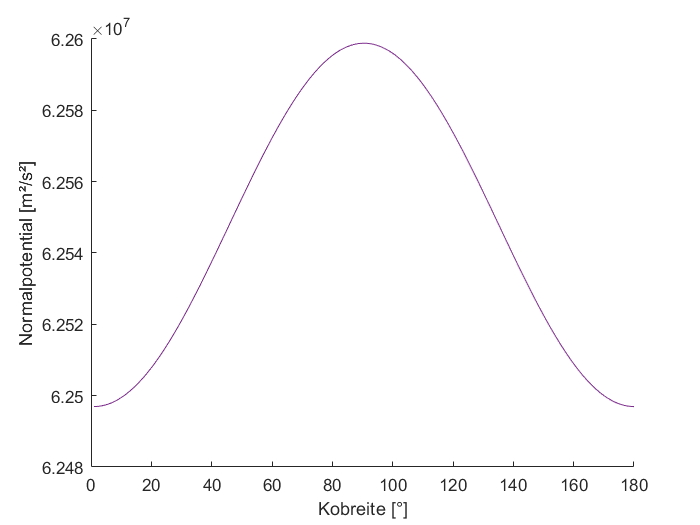
\includegraphics[scale=0.6]{ergeb.png}
\caption{Visualisierung der Ergebnisse}
\label{ergeb}
\end{figure}

In Abbildung \ref{ergeb} sieht man die Ergebnisse der Konvergenz der Reihenentwicklungen für die Entwicklungsgrade $L=2,4,6,8$ in Abhängigkeit von der Cobreite $\varphi$. Der Abbildung ist zu entnehmen, dass tatsächlich die Ergebnisse aller vier Entwicklungsgrade sich nahezu überlagern. Insofern sind keine klaren vier Kurven zu erkennen. Numerische Abweichungen treten zwar auf, sind aber dennoch sehr gering. Daraus kann man also schließen, dass die Variation des Entwicklungsgrades keinen besonders großen Einfluss auf die Ergebnisse hat. Zudem lässt sich erkennen, dass die Graphen einen Abschnitt einer harmonischen Funktion darstellen. Hierbei ist bei $90^{\circ}$, also am Äquator, das Maximum.   

\item Im zweiten Teil dieser Aufgabe wird das Somigliana-Pizzetti-Normalpotential zum Grad $L_{max}=8$ und das volle Schwerepotential (Modell EGM96 mit dem Entwicklungsgrad $L_{max} = 36$) verglichen. Hierbei werden die Entwicklungen auf einer Kugel um das Geozentrum mit Radius 6371 km ausgewertet. In farbcodierten Erdkarten werden anschließend die Potentiale, sowie deren Differenzen dargestellt. Zuletzt sollen auch die entsprechenden Werte entlang des Meridians durch Greenwich visualisiert werden. 

\begin{figure}[H]
	\centering
	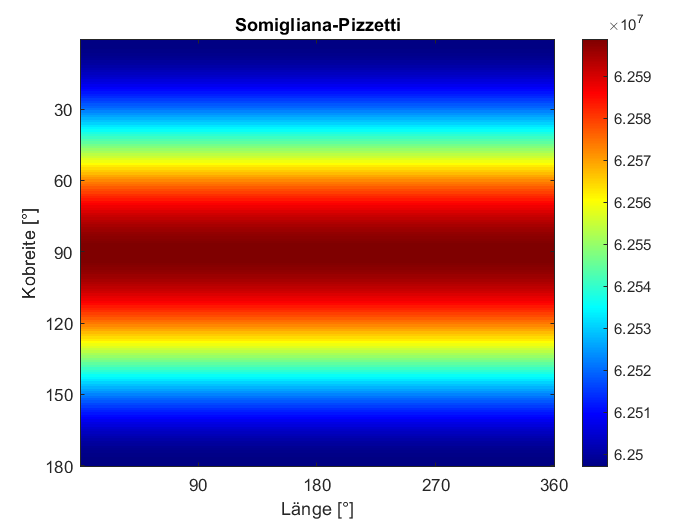
\includegraphics[scale=0.6]{SP.png}
	\caption{Somigliana-Pizzetti}
	\label{sp}
\end{figure}

Abbildung \ref{sp} stellt das Somigliana-Pizzetti-Normalpotential zum Grad $L_{max}=8$ dar.

\begin{figure}[H]
	\centering
	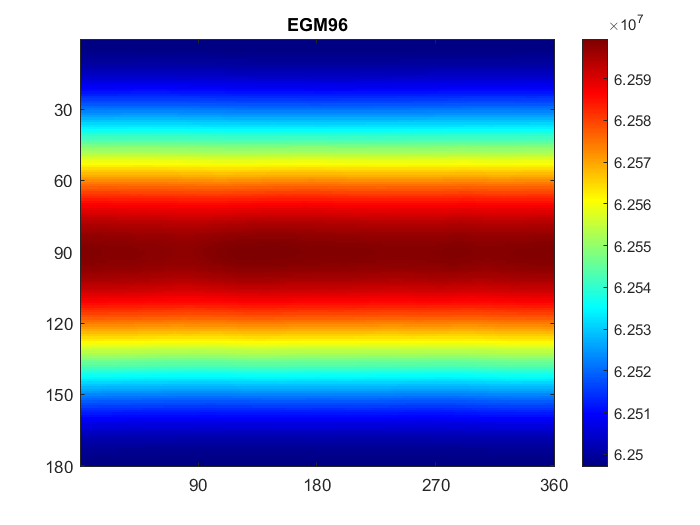
\includegraphics[scale=0.6]{egm96.png}
	\caption{EGM96}
	\label{egm96}
\end{figure}

Abbildung \ref{egm96} stellt das volle Schwerepotential zum Grad $L_{max}=36$ dar.

\begin{figure}[H]
	\centering
	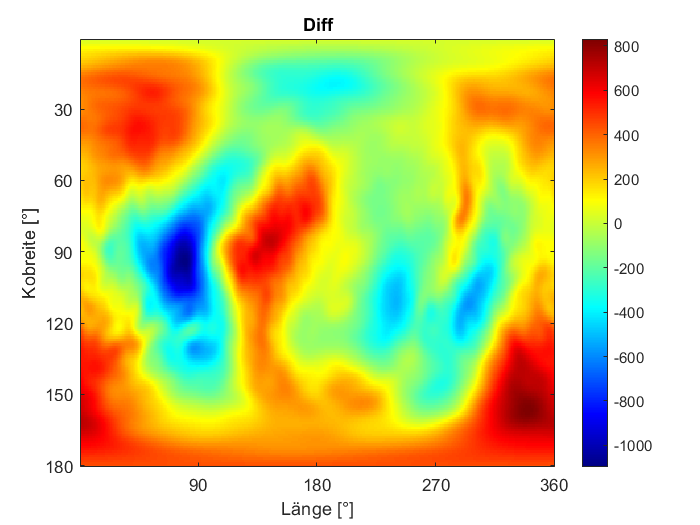
\includegraphics[scale=0.6]{diff.png}
	\caption{Differenz der beiden Potentiale}
	\label{diff}
\end{figure}

In Abbildung \ref{diff} sieht man die Differenz der beiden Potentiale dargestellt als farbcodierte Erdkarten. Bei genauerer Betrachtung fällt auf, dass die Differenz in etwa der Gestalt der Kontinente der Erde ähnelt. 

\begin{figure}[H]
	\centering
	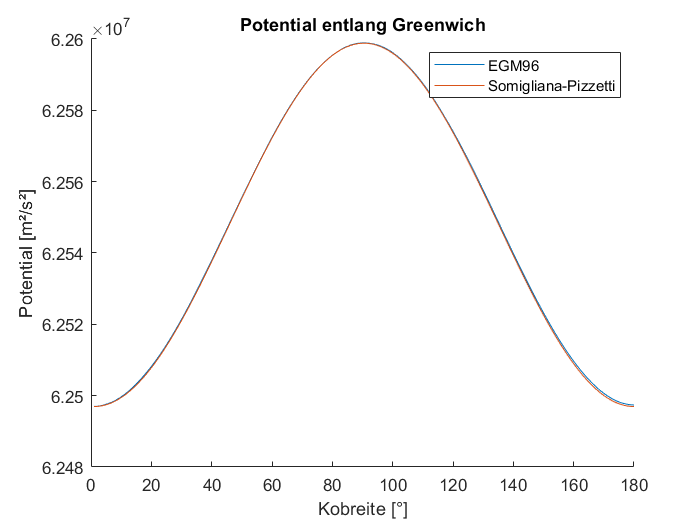
\includegraphics[scale=0.6]{greenpot.png}
	\caption{Normalpotential entlang des Greenwich Meridians}
	\label{greenpot}
\end{figure}

Abbildung \ref{greenpot} stellt die Ergebnisse entlang des Meridians durch Greenwich dar. Bemerkbar ist auch hier, dass ein Maximum am Äquator zu finden ist und, dass sich die Ergebnisse von Somigliana-Pizzetti und EGM96 grob ähneln. Differenzen finden zwar statt, sind aber nicht in einer Graphik den angezeigten Dimensionen zu erkennen. 

\begin{figure}[H]
	\centering
	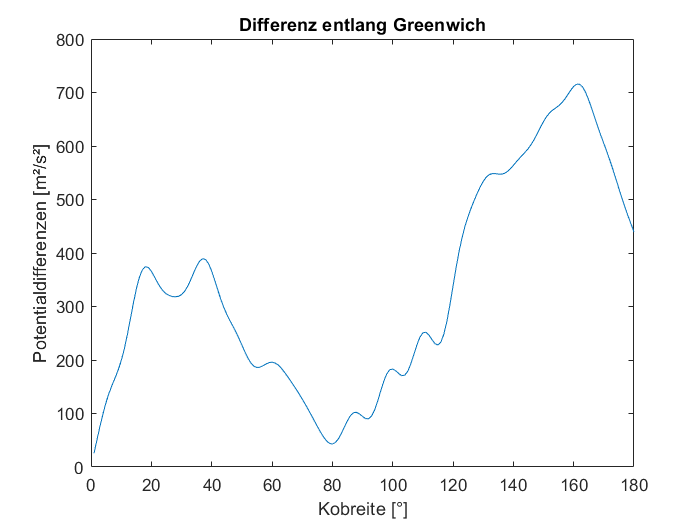
\includegraphics[scale=0.6]{greendiff.png}
	\caption{Differenzen der beiden Potentiale entlang des Greenwich Meridians}
	\label{greendiff}
\end{figure}

In Abbildung \ref{greendiff} sind nun die Differenzen der Potentiale dargestellt. Hier ist erkennbar, dass ungefähr am Äquator die Differenzen am geringsten sind. Maxima der Differenzen finden eher in Richtung der Pole statt, insbesondere nahe des Südpols. 

 
\end{enumerate}
